%!TEX root = ../dokumentation.tex

\chapter{Aufgabenstellung}\label{cha:Aufgabenstellung}
??
\chapter{D1: Aufwandsabschätzung nach der Dreipunktmethode}\label{cha:D1}
\begin{table}[H]
\centering
\caption{Dreipunktabschätzung des Aufwands der Anforderungen}
\begin{adjustbox}{width=1\textwidth, center=\textwidth}
\renewcommand{\arraystretch}{1}
\begin{tabular}{lllllll}
\textbf{Anforderung} \textbf{Optimistisch} & \textbf{Wahrscheinlich} & \textbf{Pessimistisch} & \textbf{<T>} & \textbf{sigmahoch2} & \textbf{wirklich}\\\hline
D1 & .& .& .& .& .&\\
\end{tabular}

\end{adjustbox}
\label{tbl:ConceptTPTPProductionSymbols}
\end{table}
\chapter{D2: Machbarkeitsdemonstration}\label{cha:D2}
Das Ziel der Machbarkeitsdemonstration ist es, zu zeigen, dass mit dem Modell, bestehend aus den Formeln

\begin{equation}
	\frac{\partial v}{\partial t} = -c-b*p
\end{equation}
\begin{equation}
	\frac{\partial x}{\partial t} = v
\end{equation}

die gegebene Aufgabenstellung erfüllt werden kann.

- Minimale Geschwindigkeit 0,29km/h beachten -> in m/s umrechnen \\
- Switch -> wenn Geschwindigkeit kleiner 0,29 folgt daraus Geschwindigkeit = 0 \\
- Screenshot Simulink Modell und Ergebnis\\
- R5 auch beachtet \\

\begin{figure}[H]
\centering
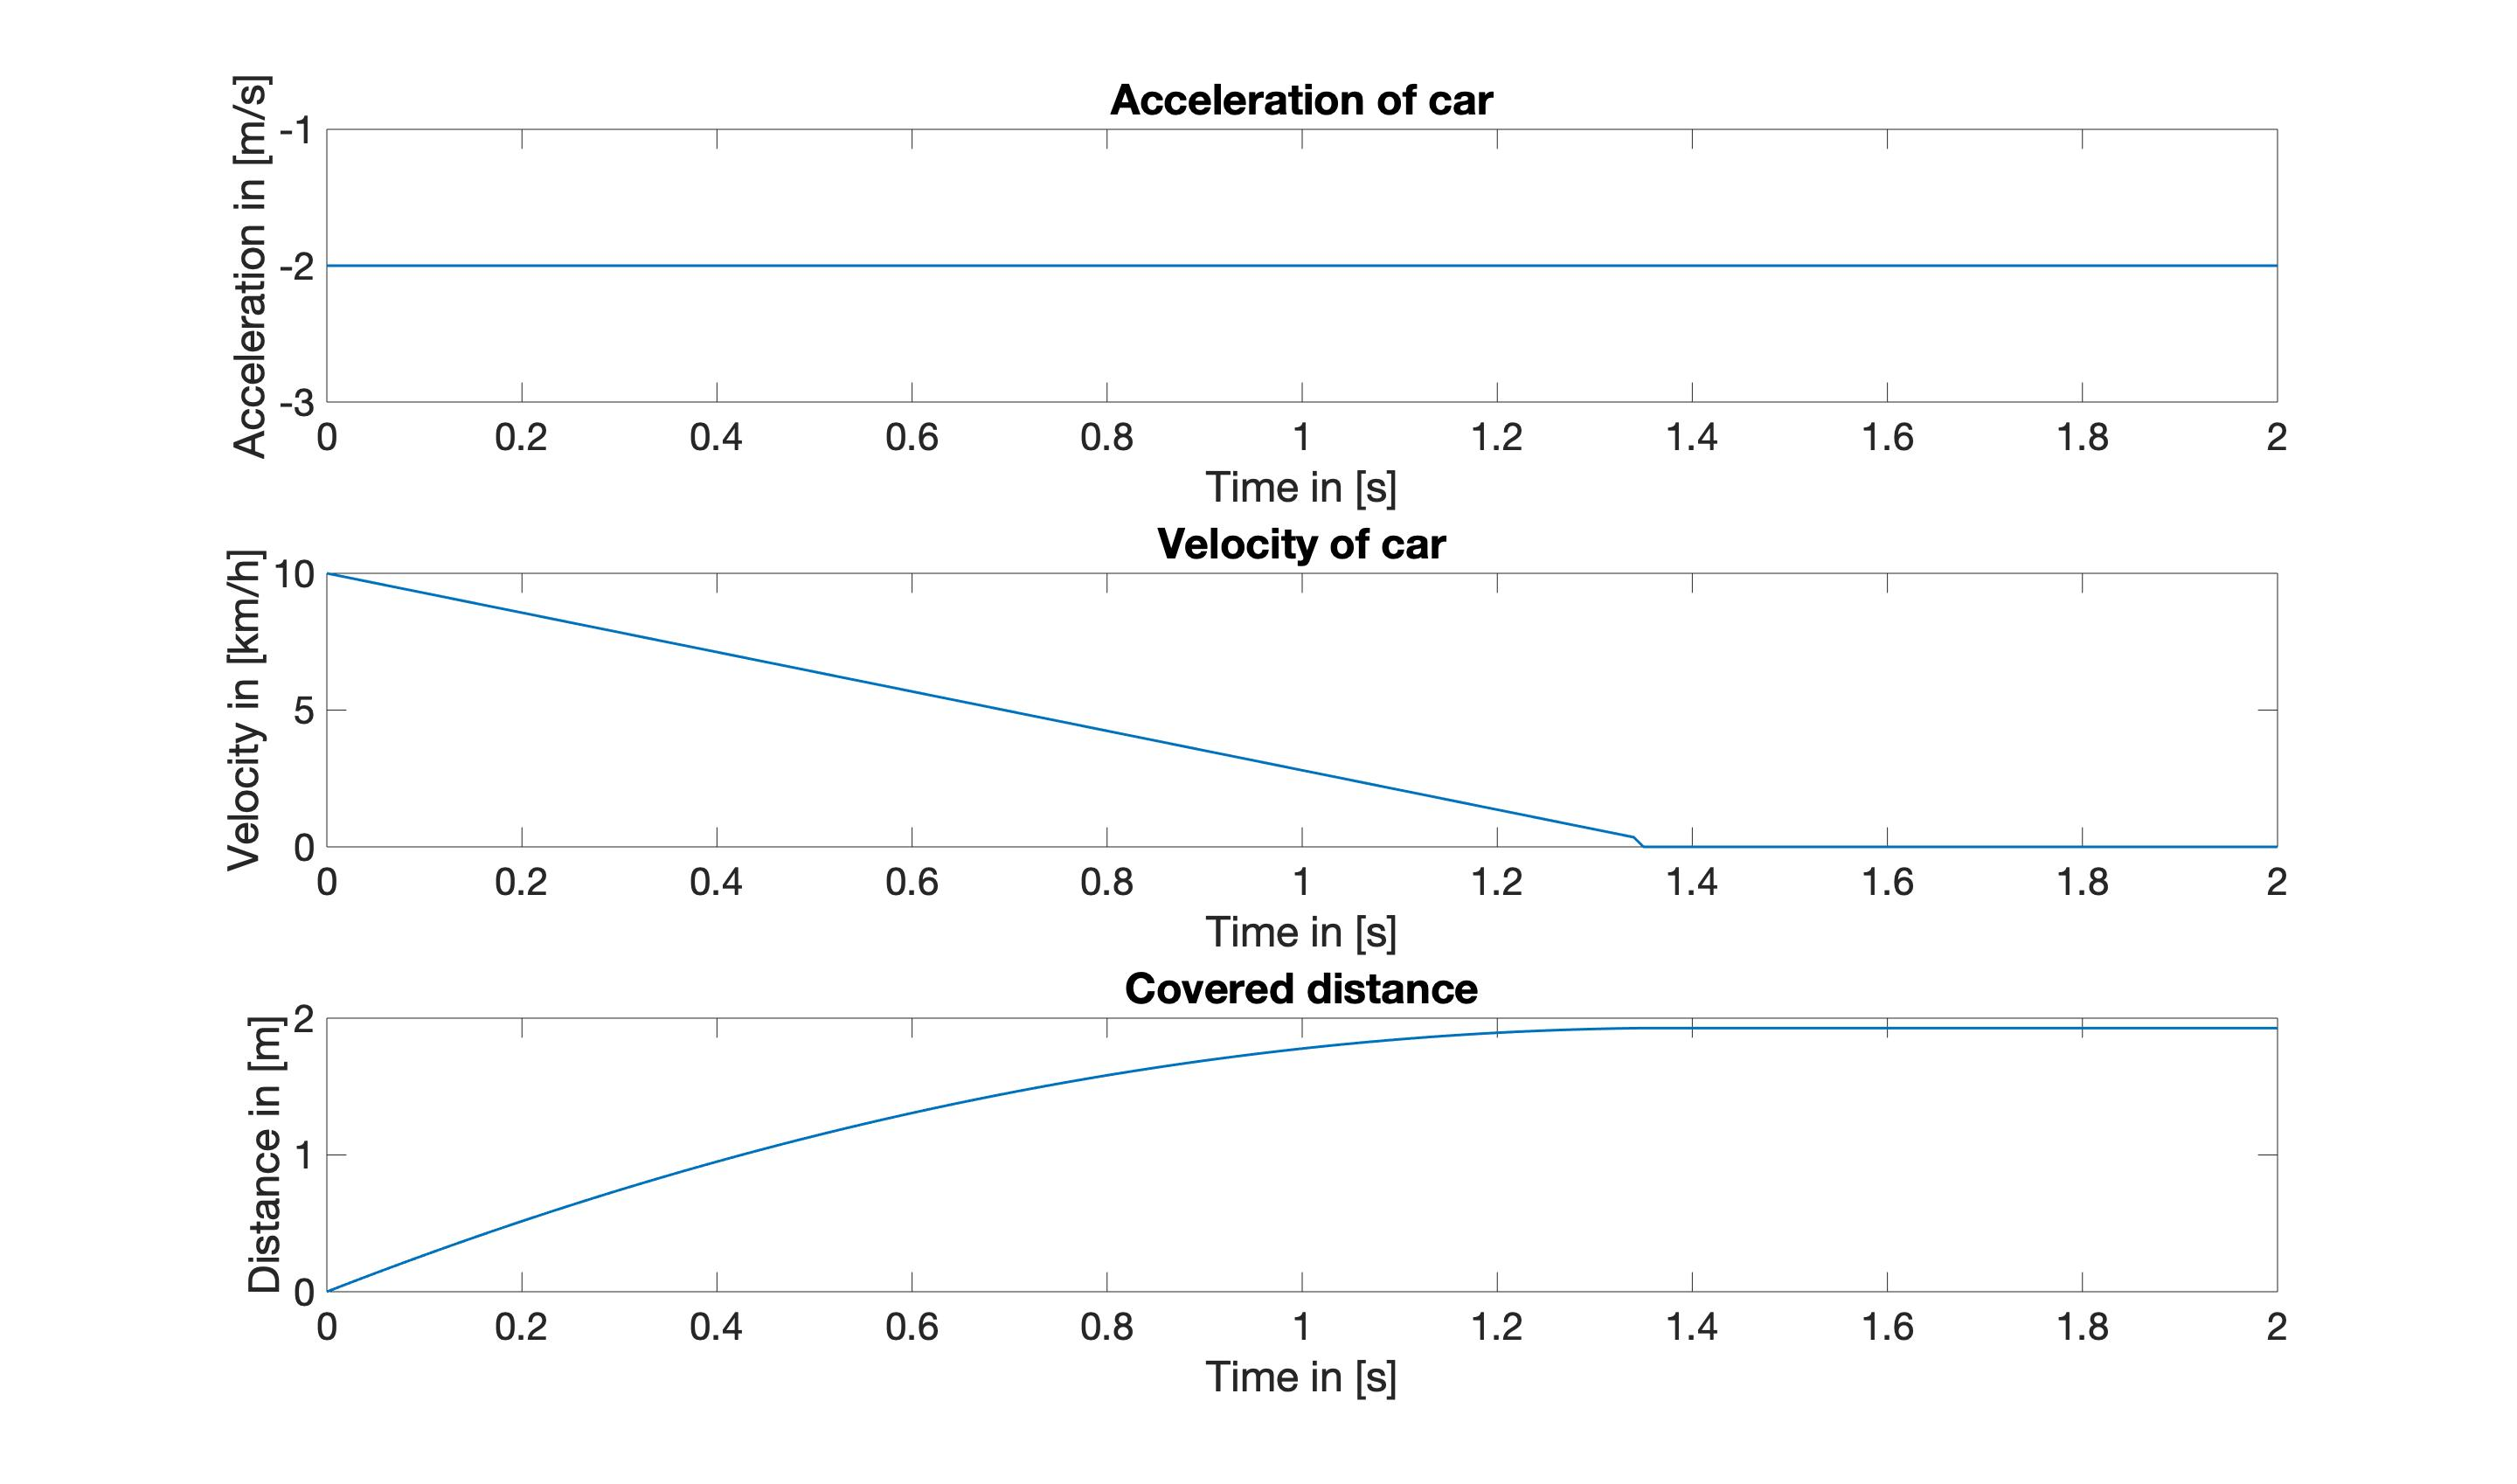
\includegraphics[width=1\textwidth]{images/D2_plot.jpg}
\caption{UML diagram of the architecture of the software tool}
\label{fig:ConceptArchitectureOverview}
\end{figure}

\begin{figure}[H]
\centering
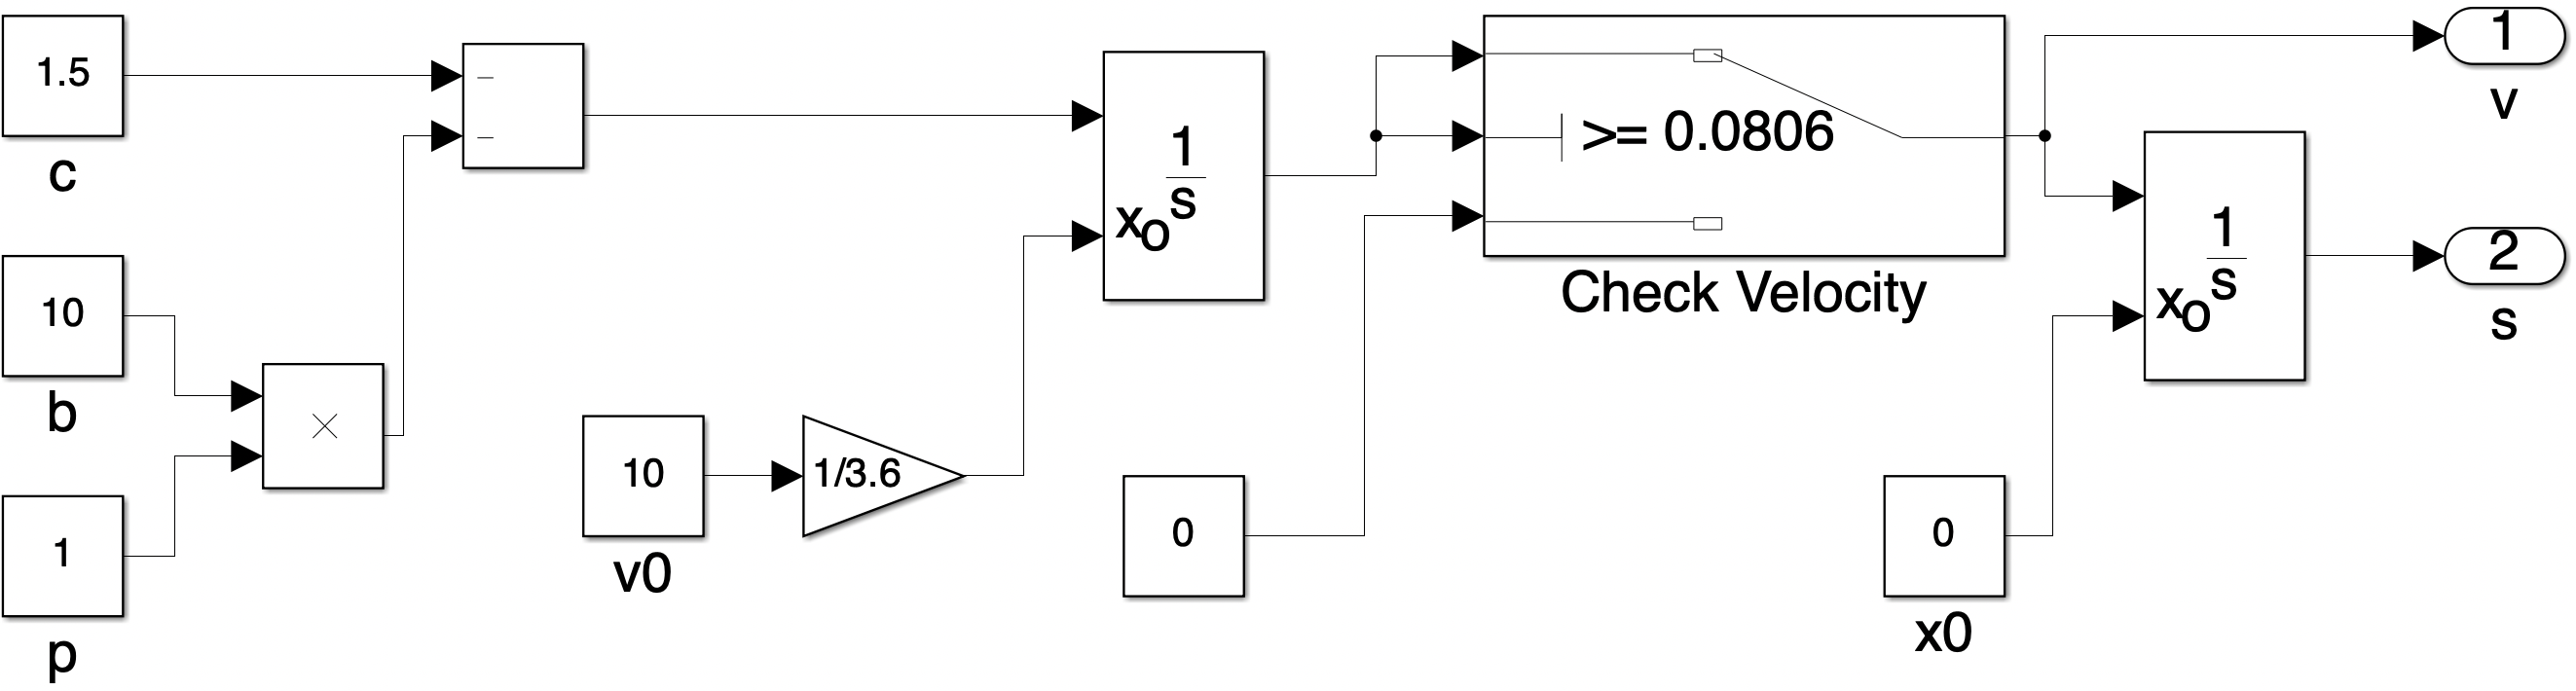
\includegraphics[width=1\textwidth]{images/D2_sim.png}
\caption{Simulink Modell der Differenzialgleichungen}
\label{fig:ConceptArchitectureOverview}
\end{figure}

\chapter{D3: Analyse des menschlichen Geschwindigkeitsprofils}\label{cha:D3}

1. Import in Matlab

2. entschieden Durchschnitt der vier Radgeschwindigkeiten zu nehmen (vllt. vor nachteile)
und so auf die Geschwindigkeit des Autos näherungsweise zu bestimmen

todo hier plot von gesamtgeschwindigkeit

idee: verzögerungsphasen extrahieren um so auf "menschliche" negative beschleunigung zu schließen
problem: verrauschte messdaten -> dadurch ständiger wehcsel positive negative beschleunigung

lösung: moving average filter zum glätten der messwerte
dann extrahieren der negativen beschleunigungen

\chapter{D4*: Betrachtung von Unebenheiten des Parkplatzes}\label{cha:D4}

\chapter{D5: Betrachtung von Unsicherheiten in der Geschwindigkeitsmessung}\label{cha:D5}
validate findings by numbers from simulation

\chapter{D6: Implementierung des Pulssignals in Simulink}\label{cha:D6}

\chapter{D7: Übernahme des Simulinkmodells nach ASCET}\label{cha:D7}

\chapter{D8: Implementierung des Pulssignals in ASCET}\label{cha:D8}

\chapter{D9: Unit-Tests für das Pulssignal in ASCET}\label{cha:D9}

\chapter{D10: Entwicklung und Druchführung von Systemtests für die ASCET Simulation}\label{cha:D10}

\chapter{D11*: Plausibilitätsprüfung gemessener Geschwindigkeiten und  Strecken gegeneinander}\label{cha:D11}

\chapter{D13*: Einfluss von Ungenauigkeiten}\label{cha:D13}

\chapter{D14*: Reflexion}\label{cha:D14}